\documentclass[12pt,hyperref={pdfpagelabels=false},notes=show]{beamer}

\usetheme[]{FFF}

% Bugfix for pdfpagelables=false
\providecommand\thispdfpagelabel[1]{}

% Standard packages

\usepackage[english,ngerman]{babel}
\usepackage[utf8]{inputenc}
\usepackage{times}

% Setup TikZ

\usepackage{tikz}
\usetikzlibrary{arrows}
\tikzstyle{block}=[draw opacity=0.7,line width=1.4cm]

% Text \us
\usepackage{textcomp}
\usepackage{mathcomp}

% Textpos
\usepackage[absolute,overlay]{textpos}
\setlength{\TPHorizModule}{\paperwidth}
\setlength{\TPVertModule}{\paperheight}

% Blitz-Symbol
\usepackage{stmaryrd}

% Tabellen
\usepackage{multirow}
\usepackage{array}
\usepackage{colortbl}
\definecolor{lightblue}{rgb}{ 0.55, 0.55, 1.00}
\definecolor{lightred}{rgb}{  1.00, 0.35, 0.35}
\definecolor{lightgreen}{rgb}{0.50, 1.00, 0.50}
\newcommand{\ccg}{\cellcolor{lightgreen}}
\newcommand{\ccr}{\cellcolor{lightred}}
\newcommand{\ccb}{\cellcolor{lightblue}}

% Listings
\usepackage{listings}

\setlength{\parindent}{0cm}

% Stroke
\usepackage{ulem}

% vc
\input{vc.tex}

%%%%%%%%%%%%%%%%%%%%%% /LAYOUT %%%%%%%%%%%%%%%%%%%%%%%%%%%%


% Author, Title, etc.

\title{Aktuelles vom Wireless Mesh Netz}

\subtitle{Erlanger Linuxtag 2016}

\author[Tim Niemeyer]{Tim Niemeyer {\tiny \textless{}tim@freifunk-franken.de\textgreater{}}\texorpdfstring{\tiny \\\\
                        https://github.com/RedDog99/vortrag-erlug2016.git\newline
                        \VCRevisionMod}{}}

\date[30.04.2016]{30.4.2016}

\newcommand{\zb}{z.\,B.\@}
\newcommand{\us}{~\textmu{}s}
\newcommand{\uv}{~\textmu{}V}
\newcommand{\ms}{~ms}

\begin{document}

\usebackgroundtemplate{
\includegraphics[height=\paperheight,width=\paperwidth]{slides_background_title}}

\beamertemplatenavigationsymbolsempty
\begin{frame}[plain,squeeze]
	\maketitle
\end{frame}\addtocounter{framenumber}{-1}

\usebackgroundtemplate{
\includegraphics[height=\paperheight,width=\paperwidth]{slides_background}}

\begin{frame}{Inhalt}
    \hspace{0.1\textwidth}
    \parbox[c][0.8\textheight][s]{0.8\textwidth}{
        \tableofcontents
    }
\end{frame}

%%%%%%%%%%%%%%%%%%%%%% CONTENT %%%%%%%%%%%%%%%%%%%%%%%%%%%%

\section{Freifunk}

\begin{frame}{Einleitung}
    \begin{itemize}
        \item Freifunk Franken ist lokaler Ableger der Freifunk-Bewegung (freifunk.net)
        \item Nicht-kommerzielle Initiative für freie Funknetzwerke\\
        \begin{itemize}
            \item[$\rightarrow$] Bürger investieren in Eigenregie Zeit, Geld und Enthusiasmus
        \end{itemize}
        \item Nicht nur \glqq{}kostenloses Internet\grqq $\Rightarrow$ \glqq{}freies Netzwerken\grqq\\
        \begin{itemize}
            \item Lokal intressante Dienste zur Verfügung stellen (Webcams)
            \item Text, Musik und Filme über das interne Freifunk-Netz übertragen
            \item Über lokale Dienste Chatten oder Telefonieren
        \end{itemize}
    \end{itemize}
\end{frame}

\begin{frame}{Wie es funktioniert}
    \begin{itemize}
        \item Freifunker stellen WLAN-Router für sich selbst und den Datentransfer der anderen Teilnehmer zur Verfügung
        \begin{itemize}
            \item ggf. mit Anschluss an das www (für VPN)
        \end{itemize}
        \item Benachbarte Router verbinden sich und spannen ein sogenanntes Mesh-Netzwerk auf
        \item Nicht benachbarte Router verbinden sich mittels VPN-Tunnel zum Freifunk
        \item Jegliche Verbindung ins www wird hierüber umgeleitet, um Risiken der Störerhaftung zu entgehen
    \end{itemize}
\end{frame}

\begin{frame}{Was braucht man?}
    \begin{itemize}
        \item Ein günstiger, unterstützter Router (ab ca. 17€)
        \item Eine spezielle Firmware
        \item Die Zustimmung zum \glqq{}Pico-Peering Agreement\grqq
        \begin{itemize}
            \item Regelwerk, das grundsätzliche Eigenschaften eines Freifunk-Netzwerkes sichert
            \begin{enumerate}
                \item Freier Transit
                \item Offene Kommunikation
                \item Keine Garantie (Haftungsausschluss)
                \item Nutzungsbestimmungen
                \item Lokale (individuelle) Zusätze
            \end{enumerate}
            \item Die Freifunk Firmware implementiert diese Grundsätze standardmäßig
        \end{itemize}
    \end{itemize}
\end{frame}


\section{Grundlagen}
\begin{frame}{}
    \begin{center}
        Grundlagen
     \end{center}
\end{frame}

\begin{frame}{Ein typisches Freifunk Netz}
    \begin{itemize}
        \item Ein Batman-Adv Netz
        \begin{itemize}
            \item[$\rightarrow$] "Wie ein großer dezentraler Switch"
        \end{itemize}
        \item VPN für die Funkinseln
        \begin{itemize}
            \item Multi-Client zu Multi-Client VPN
            \item Layer-II Netz
            \item Kein internes Routing / Forwarding
        \end{itemize}
        \item Mehrere VPN Server / Gateway
        \begin{itemize}
            \item DHCP
            \item DNS Namensauflösung
            \item Gateway zum Internet / ICVPN
        \end{itemize}
        \item Monitoring
        \begin{itemize}
            \item Karte aller Knoten
        \end{itemize}
    \end{itemize}
\end{frame}

\begin{frame}{Ein typisches Freifunk Netz}
    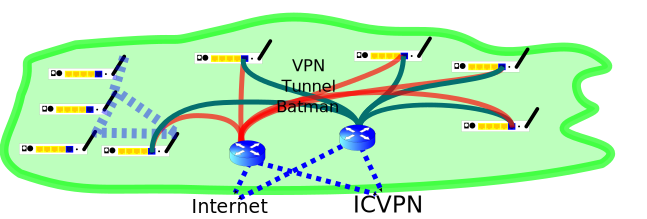
\includegraphics[width=\textwidth]{img/svg/freifunk_konzepte_alt.pdf}
\end{frame}

\begin{frame}{Freifunk Franken Netz}
    \includegraphics[width=\textwidth]{img/svg/freifunk_konzepte.pdf}

    \begin{itemize}
        \item Mehrere Layer-2 Inseln (Hoods)
        \item Verbindung per Layer-3
        \item Dezentrale Gateways
    \end{itemize}
\end{frame}

\begin{frame}{Knoten VPN}
    \begin{itemize}
        \item Verwendetes VPN: fastd
        \begin{itemize}
            \item n:m VPN
        \end{itemize}
        \item Endpunkt Vermittlung über KeyXchange:
        \begin{itemize}
            \item Zentrale Webseite \only<2-3>{{\color{red}Problem!}}
            \item Knoten meldet sich mit Standort
            \item Geographisch nächste Hood wird zugewiesen (voronoi)
            \item Client bekommt Liste aller Server der Hood
        \end{itemize}
        \item<3> Keine weitere Unterscheidung zu welcher Hood der Knoten gehört
        \item<3> {\color{red}Problem!} Funk Verbindung zwischen den Hoods
    \end{itemize}
\end{frame}

\begin{frame}{VPN Server}
    \begin{itemize}
        \item VPN Server: In jeder Hood gibt es mehrere davon
        \item Hoodzuweisung manuell im KeyXchange
        \item DHCP
        \begin{itemize}
            \item Aktuell ausschließlich IPv4
            \item Unterschiedliche Latenzen: Ungleiche Server Auslastung
            \begin{itemize}
                \item[$\rightarrow$] Batman-Adv GW Selection
                \item Anpassung nach Traffic Auslastung
            \end{itemize}
        \end{itemize}
        \item DNS Namesauflösung
        \item Policy base routing
        \item VPN (GRE) Tunnel zu anderen Gateways
        \begin{itemize}
            \item OLSR Routing
        \end{itemize}
    \end{itemize}
\end{frame}

\begin{frame}{Gateways}
    \begin{itemize}
        \item Verbindet Freifunk und Internet
        \item IPv4 NAT (oft übers Ausland) ins Internet
        \item Announced 0.0.0.0/0 via OLSR
        \begin{itemize}
            \item Dynamic Gateway Plugin
            \item VPN Server können diese Routen nutzen
        \end{itemize}
        \item Routing Metrik ohne Traffic/Bandbreite
        \item<2> {\color{red}Problem!} Ungleiche Traffic Verteilung
    \end{itemize}
\end{frame}

\section{Knoten}
\begin{frame}{}
    \begin{center}
        Freifunk Franken Knoten
     \end{center}
\end{frame}

\begin{frame}{Freifunk Franken Knoten}
    \begin{center}
        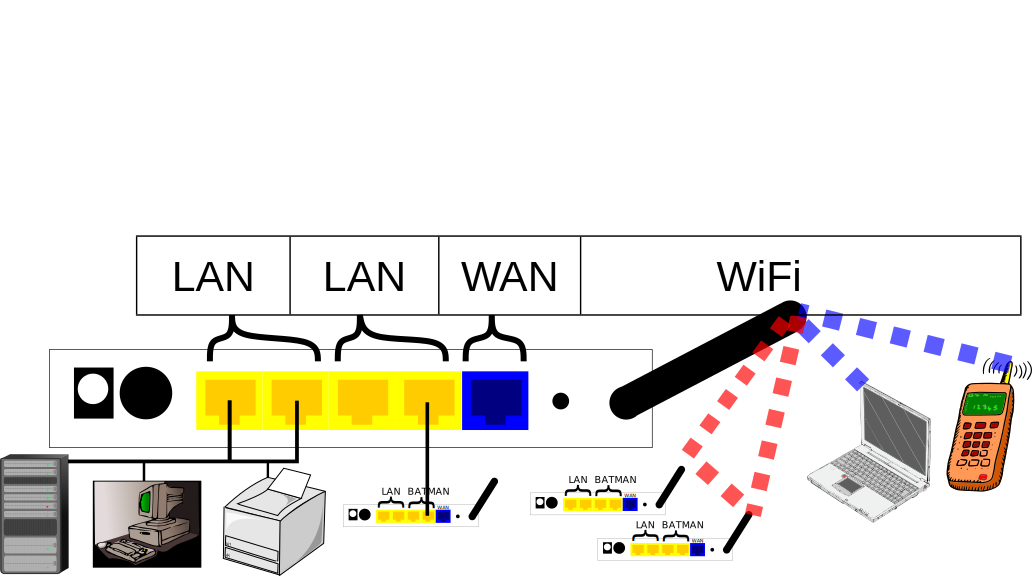
\includegraphics[width=0.75\textwidth]{img/svg/anschluesse.pdf}
    \end{center}
    \begin{tabular}{ll}
        LAN, Access-Point: & Client-Ports\footnote{,,Wie ein großer Switch''} \\
        Batman, Ad-Hoc: & Mesh-Netz \\
        WAN: & VPN Zugang \\
    \end{tabular}
\end{frame}

\begin{frame}{Interner Aufbau}
    \begin{itemize}
        \item OpenWrt
        \item Batman-Adv
        \item Fastd Client
        \item Monitoring Daten (Nodewatcher / Alfred)
        \item .. kleinere Tools / Configs / Skripte
    \end{itemize}

    \renewcommand{\arraystretch}{1.5}
    \begin{tabular}{|c|c|c|c|c|c|c|} \hline
         \multicolumn{7}{|c|}{Bridge} \\ \hline
         \multirow{2}{*}{Managed} &
         \multicolumn{4}{c|}{B.A.T.M.A.N} &
         \multicolumn{2}{c|}{\multirow{2}{*}{Client-VLan}} \\ \cline{2-5}
         & Ad-Hoc & VPN & \multicolumn{2}{c|}{Node-VLan} & \multicolumn{2}{c|}{} \\ \hline
         \multicolumn{2}{|c|}{WiFi} & WAN & LAN1 & LAN2 &
         LAN3 & LAN4 \\ \hline
    \end{tabular}
\end{frame}

\begin{frame}{Freifunk Knoten}
    \only<1>{
        \begin{itemize}
            \item Vergibt ein spezielles IPv6 Prefix: fdff:0::
            \begin{itemize}
                \item fdff:0::1
                \item fdff:0::\$\{MAC\}
                \item fdff:0::\$\{Link-Local suffix\}
            \end{itemize}
            \item Webinterface
            \item Konfiguration am Gerät
            \begin{itemize}
                \item Passwort
                \item Knoten-Name
                \item Beschreibung
                \item Ansprechpartner
                \item Standort
            \end{itemize}
        \end{itemize}
    }
    \only<2-4>{\hspace{-0.04\textwidth}
        \noindent\fbox{\noindent
            \only<2>{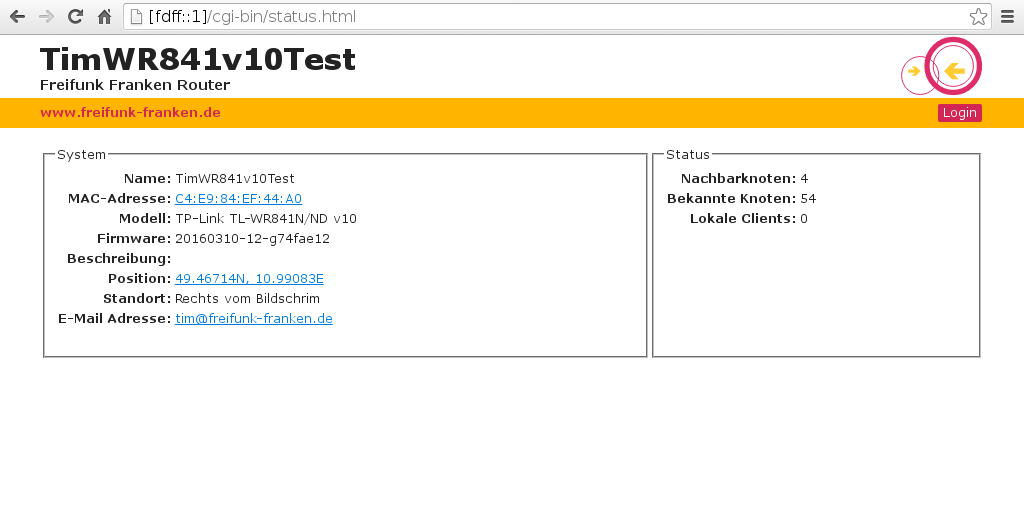
\includegraphics[width=1.03\dimexpr\textwidth-2\fboxsep-2\fboxrule\relax]{img/web-if-1.png}}%
            \only<3>{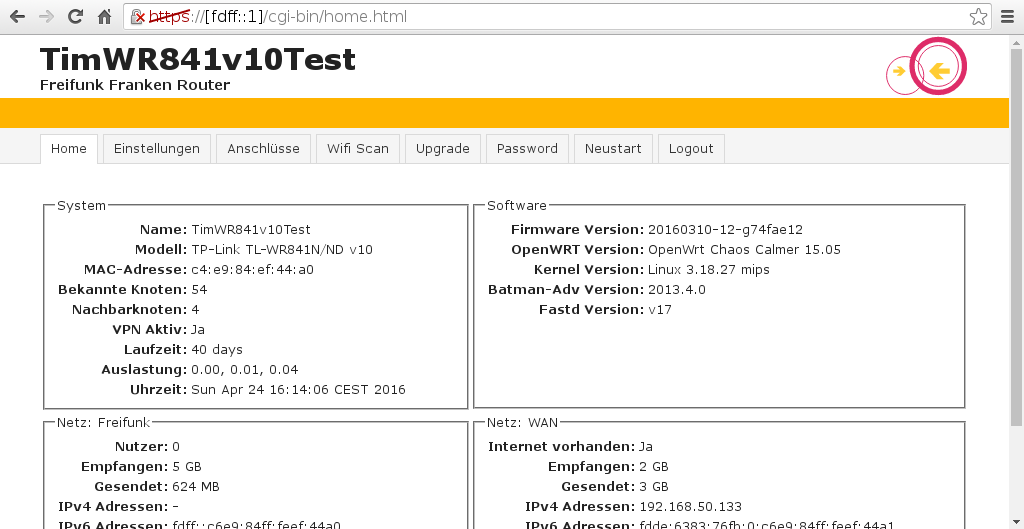
\includegraphics[width=1.03\dimexpr\textwidth-2\fboxsep-2\fboxrule\relax]{img/web-if-2.png}}%
            \only<4>{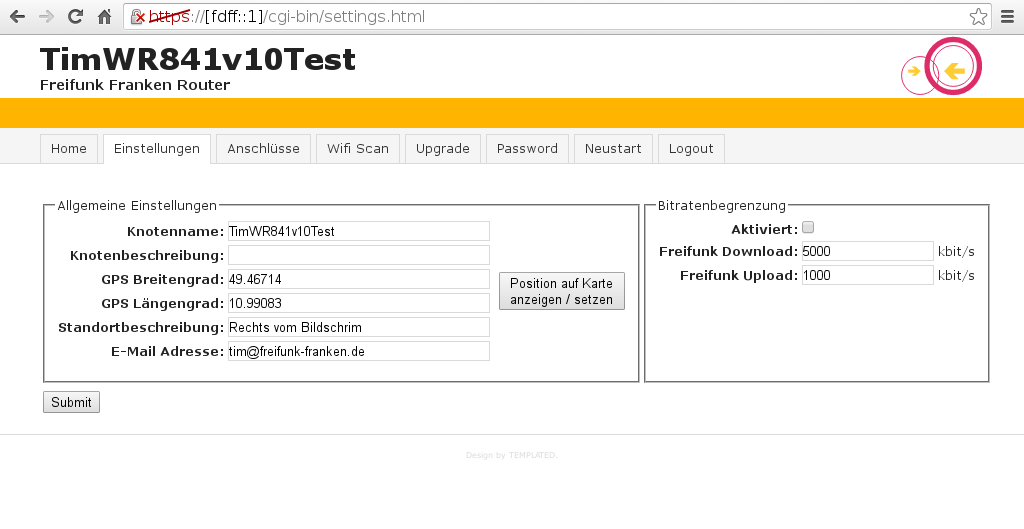
\includegraphics[width=1.03\dimexpr\textwidth-2\fboxsep-2\fboxrule\relax]{img/web-if-3.png}}%
        }
    }
\end{frame}

\section{Netz}
\begin{frame}{}
    \begin{center}
        Das Netz
     \end{center}
\end{frame}

\begin{frame}{Knoten VPN}
    \begin{itemize}
        \item Verwendetes VPN: fastd
        \begin{itemize}
            \item {\small{}Wir nutzen keine Verschlüsselung (! :-O)}
        \end{itemize}
        \item Endpunkt Vermittlung über KeyXchange:
        \begin{itemize}
            \item Zentrale Webseite \only<2-3>{{\color{red}Problem!}}
            \item Knoten meldet sich mit Standort
            \item Geographisch nächste Hood wird zugewiesen (voronoi)
            \item Client bekommt Liste aller Server der Hood
        \end{itemize}
        \item<3> Keine weitere Unterscheidung zu welcher Hood der Knoten gehört
        \item<3> {\color{red}Problem!} Funk Verbindung zwischen den Hoods
    \end{itemize}
\end{frame}

\begin{frame}{VPN Server}
    \begin{itemize}
        \item VPN Server: In jeder Hood gibt es mehrere davon
        \item Hoodzuweisung manuell im KeyXchange
        \item DHCP
        \begin{itemize}
            \item Aktuell ausschließlich IPv4
            \item Unterschiedliche Latenzen: Ungleiche Server Auslastung
            \begin{itemize}
                \item[$\rightarrow$] Batman-Adv GW Selection
                \item Anpassung nach Traffic Auslastung
            \end{itemize}
        \end{itemize}
        \item DNS Namesauflösung
        \item Policy base routing
        \item VPN (GRE) Tunnel zu anderen Gateways
        \item OLSR
        \begin{itemize}
            \item Routing zu anderen Gateways
        \end{itemize}
    \end{itemize}
\end{frame}

\begin{frame}{Gateways}
    \begin{itemize}
        \item Verbindet Freifunk und Internet
        \item IPv4 NAT (oft übers Ausland) ins Internet
        \item Announced 0.0.0.0/0 via OLSR
        \begin{itemize}
            \item Dynamic Gateway Plugin
            \item VPN Server können diese Routen nutzen
        \end{itemize}
        \item Routing Metrik ohne Traffic/Bandbreite
        \item<2> {\color{red}Problem!} Ungleiche Traffic Verteilung
    \end{itemize}
\end{frame}

\section{Dienste}
\begin{frame}{}
    \begin{center}
        Dienste im Netz
     \end{center}
\end{frame}

\begin{frame}{Monitoring}
    \begin{itemize}
        \item Alfred
        \begin{itemize}
            \item XML
            \item alle 5 Minuten
            \item Multicast
        \end{itemize}
        \item Multicast Daten können auf mehreren Gateways gelesen werden
        \item Die Daten können von dort an eine zentrale Webseite (Karte, etc.) geschickt werden
    \end{itemize}
    \begin{itemize}
        \item Alfred-Legacy Provider
        \item Alfred-Proxy
        \item beides nur auf dem Netmon-Server
    \end{itemize}
\end{frame}

\begin{frame}{Domain-Name-System}
    \begin{itemize}
        \item fff.community
        \begin{itemize}
            \item Langer Name, aber
            \item Keine Kollision
        \end{itemize}
        \item Mehrere DNS Server
        \item Zonen-Synchronisation über dig axfr
        \item Subdelegation an synchronisierte Hosts möglich
        \item Automatisierte reverse delegation
    \end{itemize}
\end{frame}

\begin{frame}{Firmware Bau}
    \begin{itemize}
        \item Basiert auf OpenWrt
        \item ,,Eigenes'' Framework (Buildscript)
        \item Zentrales ,,files'' Verzeichnis
        \item Board-Support-Packages
        \begin{itemize}
            \item Ein .config
            \item Überschreibende ,,files''
        \end{itemize}
        \item Template System für versch. Communities
        \item Versionierung:
            \begin{itemize}
                \item YYYYmmDD
                \item ...
            \end{itemize}
    \end{itemize}
\end{frame}

\section{Zusammenfassung}
\begin{frame}{}
    \begin{center}
        Zusammenfassung
     \end{center}
\end{frame}

\begin{frame}{Freifunk V1}
    \begin{itemize}
        \item Aktuelle (!) veraltete (!) Freifunk Firmware
        \begin{itemize}
            \item VPN Schlüsseltausch über zentrales Tool
            \item Manuelle Zuweisung der VPN Server
            \item Keine Anpassung an Firmware
            \item[$\rightarrow$] Loop durch versehentliches Meshing
        \end{itemize}
        \item Einseitiges Peering (viel Ausnutzung)
        \begin{itemize}
            \item[$\rightarrow$] Viele Router-Aufsteller
            \item[$\rightarrow$] Zu wenig Vernetzung
        \end{itemize}
    \end{itemize}
\end{frame}

\begin{frame}{Freifunk V2}
    \begin{itemize}
        \item Zukünftige (?) Freifunk Firmware
        \begin{itemize}
            \item VPN Schlüsseltausch über zentrales Tool
            \item Manuelle Zuweisung der VPN Server
            \item Theoretisch keine Loops
            \item[$\rightarrow$] Komplexität (viel) zu hoch
        \end{itemize}
        \item Einseitiges Peering (viel Ausnutzung)
        \begin{itemize}
            \item[$\rightarrow$] Viele Router-Aufsteller
            \item[$\rightarrow$] Zu wenig Vernetzung
        \end{itemize}
    \end{itemize}
\end{frame}

\begin{frame}{Freifunk V3}
    \begin{itemize}
        \item Zukünftige Freifunk Vernetzung
        \begin{itemize}
            \item Kein automatisches Peering
            \item[$\rightarrow$] Weniger Router-Aufstellern
        \end{itemize}
        \item Kaum Doku
        \item Manuelles Peering nötig
        \begin{itemize}
            \item Viel (soziale) Vernetzung
            \item Wecken von Potential
        \end{itemize}
        \item Layer 3 Routing
        \begin{itemize}
            \item Sehr hohe Performance
            \item Leichtes Debuggen
            \item Standard Komponenten
        \end{itemize}
    \end{itemize}
\end{frame}


\section*{}
\begin{frame}{Ende}
    \begin{center}
        Vielen Dank für Eure Aufmerksamkeit	...
     \end{center}
\end{frame}\addtocounter{framenumber}{-1}
	
%%%%%%%%%%%%%%%%%%%%%% /CONTENT %%%%%%%%%%%%%%%%%%%%%%%%%%%%

\end{document}
